%%%%%%%%%%%%%%%%%%%%%%%%%%%%%%%%%%%%%%%%%%%%%%%%%%%%%%%%%%%%%%%%%%%%%%%%%%%%%%%%%%%%%%%%%%%%%%%%%%%%

\chapter{Details on the turbulent gas structure in the centers of \ngc253 and the Milky Way}
\chaptermark{Details on turbulent gas}
\label{appendix: dendro}

%%%%%%%%%%%%%%%%%%%%%%%%%%%%%%%%%%%%%%%%%%%%%%%%%%%%%%%%%%%%%%%%%%%%%%%%%%%%%%%%%%%%%%%%%%%%%%%%%%%%


\section{Definition of structure properties}
\label{appendix: dendro: structure definition}

The exact definition of size and line width of a structure can influence the derived relation \citep[e.g.][]{2002ApJ...570..734B,2010ApJ...712.1049S}. For the basic quantities size and line width of a structure multiple valid definitions are possible. In this section, we explore the effect of these different definitions on derived properties such as the size--line width relation.

%%%%%%%%%%%%%%%%%%%%%%%%%%%%%%%%%%%%%%%%%%%%%%%%%%%%%%%%%%%%%%%%%%%%%%%%%%%%%%%%%%%%%%%%%%%%%%%%%%%%

\subsection{Structure size}
\label{appendix: dendro: size definition}

The derivation of a linear size quantity for an \astrodendro structure is always limited to the information drawn from the 2D projection of a 3D cloud onto the plane of the sky.
The cloud extent along radial direction is not known and must be assumed to be similar to the projected extent.
The size of a structure can then either be defined by its linear extent in some direction(s) or via the covered area.
The former approach is limited to probing the size in (typically) two directions whereas the latter takes the often complex shape into account.
A definition of size using the projected area, however, does not account for the distribution of gas within a structure. In an extreme case, 99\% of the mass might be inside 1\% of the area and a good definition of structure size should come up with a size much smaller then the total extend of the cloud.
The size definition \astrodendro (\texttt{radius}) tries to acknowledge both shape and distribution by defining ``size'' as the mean structure radius of the intensity-weighted second moment map. Mean structure radius is defined as the mean of major axis in the direction of greatest elongation and the minor axis perpendicular to the major axis.
In this comparison, we denote this definition as R$_\mathrm{astrodendro}$.
Alternatively, the size R$_\mathrm{ellipse}$ can be defined as the mean radius of an ellipse with equal area to the projected structure fitted to the structure. This ellipse is calculated by \astrodendro as the \texttt{area\_ellipse} quantity and useful for plotting structures on top of the map.
The most simple size estimation is the radius R$_\mathrm{circular} = \sqrt{\mathrm{A}/\pi}$ as the radius corresponding to the total projected area A of a structure.

In Figure~\ref{dendro: figure: A} (left), we compare these estimates against R$_\mathrm{astrodendro}$ for \co32 in NGC253.
R$_\mathrm{astrodendro}$ and R$_\mathrm{ellipse}$ result in very similar sizes whereas R$_\mathrm{circular}$ yields size a factor $\sim 2$ larger.
Over $\GTR 2$ order of magnitude all definitions lie very close to parallel to each other which implies that only the normalisation of derived properties will change across size definitions.
Hence, we use R$_\mathrm{astrodendro}$ as the definition of size in this work since it is also used in the literature.
Note that in any case, a disambiguity of the phrase ``size'' as radius or diameter persists. Structure sizes smaller than the resolution are thus not the problem they at first appear to be.

%%%%%%%%%%%%%%%%%%%%%%%%%%%%%%%%%%%%%%%%%%%%%%%%%%%%%%%%%%%%%%%%%%%%%%%%%%%%%%%%%%%%%%%%%%%%%%%%%%%%

\begin{figure*}
    \centering
    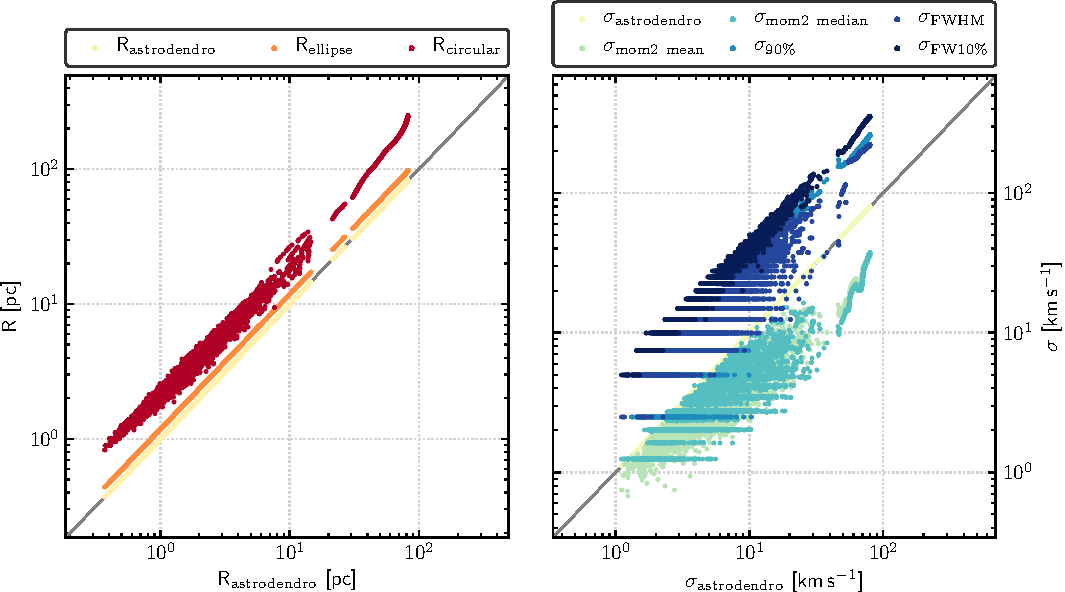
\includegraphics[width=\linewidth]{images/chapters/papers/dendro/dendro_figA}
    \caption[Comparison of definitions for structure size and line width]{Comparison of different definitions for structure size (\emph{left}) and line width (\emph{right}). 
    The suffix astrodendro refers to the quantities calculated by \astrodendro directly as described in Section~\ref{dendro: section: dendrogram}.
    For details on the other definitions for size and line width see Appendix~\ref{appendix: dendro: size definition} and \ref{appendix: dendro: line width definition}, respectively.
    Quantisation apparent in some line width definitions follows directly from the discrete channel structure of the data cubes.
    }
    \label{dendro: figure: A}
\end{figure*}

%%%%%%%%%%%%%%%%%%%%%%%%%%%%%%%%%%%%%%%%%%%%%%%%%%%%%%%%%%%%%%%%%%%%%%%%%%%%%%%%%%%%%%%%%%%%%%%%%%%%

\subsection{Structure line width}
\label{appendix: dendro: line width definition}

Similarly to size, the line width can be defined in various ways that take the spectral distribution of gas within a structure into account.
$\sigma_\mathrm{astrodendro}$ is \texttt{v\_rms} quantity in \astrodendro that corresponds to the square-root of the moment 2 map.
We compare this definition to the mean and median over the pixels of an independently calculated intensity-weighted moment 2 map of the structure. These are labeled $\sigma_\mathrm{mom2\ mean}$ and $\sigma_\mathrm{mom2\ median}$, respectively.
We also test approaches to capture the spectral structure of an \astrodendro structure. Note that these definitions do not take the intensity distribution into account as the moment-based approaches do.
$\sigma_\mathrm{90\%}$ is the line width corresponding to 90\% of the emission in the spectrum of a structure.
line width can also be defined as the width at half (FWHM) or 10\% (FW10\%) of the maximum of the structure spectrum.

Figure~\ref{dendro: figure: A} (right) shows the comparison of these six line width definitions for \co32 in NGC253.
There is $\sim 1$ order of magnitude difference between the most extreme definitions (moment-based and FW10\%) with $\sigma_\mathrm{astrodendro}$ sitting in the middle.
The definitions in which line width is defined as a difference between image channels (FWHM and FW10\%) are quantized in multiples of the channel width of 2.5\,\kms. For the moment 2 median quantization on a smaller scale occurs because of the intensity-weighted moment 2 map calculation.
Aside from the highest line width structures (that happen to be the trunks and lowest branches in the dendrogram tree), the different definitions lie approximately parallel to each other indicating that only the normalization changes. Choosing a different definition of line width will thus not distort derived relations but merely shift them.
We use the \astrodendro definition of line width in this work since it falls in between the extremes and has been used in many cases in the literature.


%%%%%%%%%%%%%%%%%%%%%%%%%%%%%%%%%%%%%%%%%%%%%%%%%%%%%%%%%%%%%%%%%%%%%%%%%%%%%%%%%%%%%%%%%%%%%%%%%%%%

\section{Size -- mass relation}
\label{appendix: dendro: size mass}

In Figure~\ref{dendro: figure: B}, we show the size--mass relation. This figure is derived from Figure~\ref{dendro: figure: 3} by applying the conversion factors listed in Table~\ref{dendro: table: conversion factors}.

\begin{figure*}
    \centering
    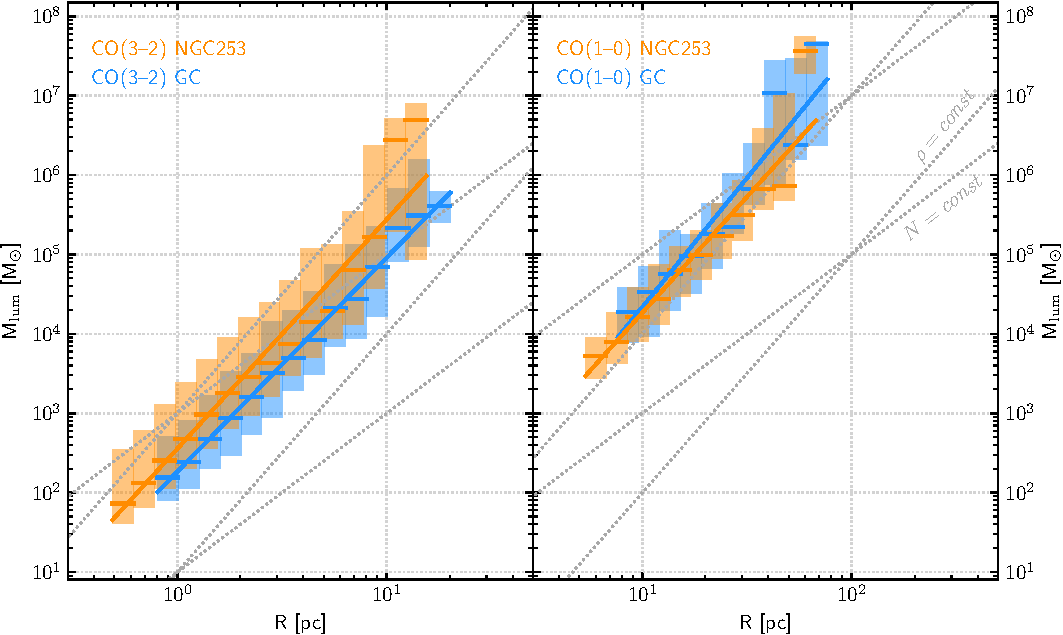
\includegraphics[width=\textwidth]{images/chapters/papers/dendro/dendro_figB}
    \caption[Size--mass relation]{Relation between dendrogram structure size and mass for \co32 (\emph{left}) and \co10 (\emph{right}) in NGC253 and the GC. Horizontal lines indicate the median of the distribution of masses (colored bars) in each bin. The power law fits (solid lines) correspond to those to the size--luminosity relation (Table~\ref{dendro: table: 2}). The masses are derived according to the conversion factors listed in Table~\ref{dendro: table: conversion factors}.
    In each panel, two lines of constant surface density $N$ ($M \propto R^2$) and constant volume density $\rho$ ($M \propto R^3$) are shown for reference.
    \label{dendro: figure: B}}
\end{figure*}



%%%%%%%%%%%%%%%%%%%%%%%%%%%%%%%%%%%%%%%%%%%%%%%%%%%%%%%%%%%%%%%%%%%%%%%%%%%%%%%%%%%%%%%%%%%%%%%%%%%%

\section{Density and mass probability density function}
\label{appendix: dendro: mass density structure}

With the structure identification in place, we can compare further properties of the structures to infer possible deviations between NGC253 and the GC. 
Figure~\ref{dendro: figure: C} shows the probability density functions (PDFs) for column density, volume density and mass.

Whereas column density and mass only rely on the assumption of a conversion factor (X$_\mathrm{CO}$ or $\alpha_\mathrm{CO}$), the volume density further requires an assumption about the 3D distribution within a structure since the gas distribution in the radial direction is not known from observations. As the most simple assumption, we assume the clouds to be as extended radially as they are in the plane of the sky. The ``depth'' of a cloud is thus equal to the diameter and its volume is $V = \frac{4}{3} \pi R^3$. The volume density simply is $n = (M_\mathrm{H_2}+M_\mathrm{He})/V$ and expressed in atoms per cm$^3$.

\begin{figure*}
    \centering
    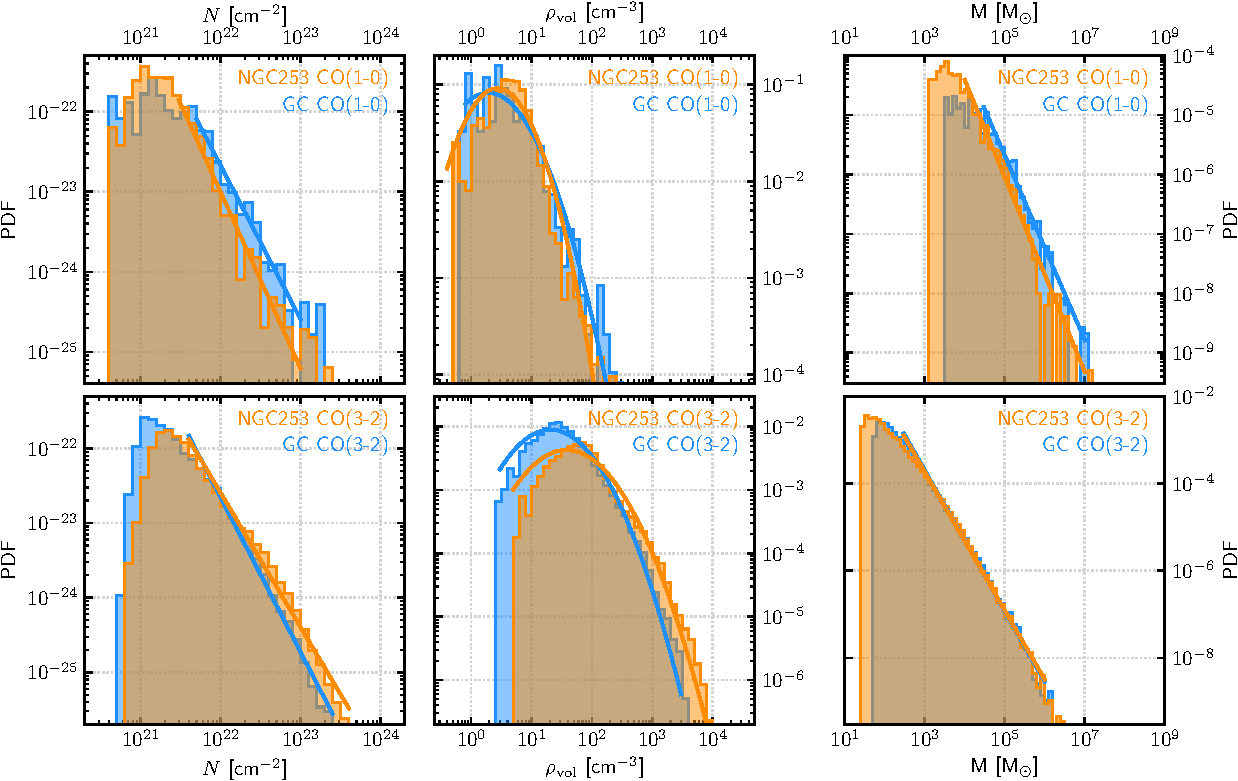
\includegraphics[width=\textwidth]{images/chapters/papers/dendro/dendro_figC}
    \caption[Column density, volume density and mass PDFs]{Probability density functions for column density (\emph{left}), volume density (\emph{center}) and cloud mass (\emph{right}) for \co10 (\emph{top}) and \co32 (\emph{bottom}). We fit the column density and mass PDFs with power laws and the volume density PDFs with lognormal distributions. The fit results are reported in Table~\ref{dendro: table: 3}.
    \label{dendro: figure: C}}
\end{figure*}

\begin{table}
    \centering
    \begin{threeparttable}
        \caption[Results of the fits to column density, volume density and mass PDFs]{Results for the lognormal fits to the volume density PDFs and power law fits to the mass PDFs shown in Figure~\ref{dendro: figure: C}.
        \label{dendro: table: 3}}
        
        \begin{tabular}{lcccccccc}
            \toprule
            source & line & \multicolumn{2}{c}{column density} & \multicolumn{2}{c}{volume density} & \multicolumn{2}{c}{mass}\\
            && $\gamma$ & $a$\ & $\mu$ & $\sigma$ & $\gamma$ & $a$\\
            && (1) & (2) & (3) & (4) & (5) & (6)\\
            \midrule
NGC253 & CO(1--0) & $-2.20$ & $25.34$ & $1.97$ & $0.98$ & $-1.64$ & $2.14$ \\
GC     & CO(1--0) & $-1.92$ & $19.59$ & $2.12$ & $1.21$ & $-1.55$ & $2.09$ \\
NGC253 & CO(3--2) & $-1.80$ & $17.04$ & $5.07$ & $1.20$ & $-1.59$ & $1.03$ \\
GC     & CO(3--2) & $-2.07$ & $22.97$ & $4.32$ & $1.14$ & $-1.61$ & $1.14$ \\
            \bottomrule
        \end{tabular}
        \vspace{0.5em}
	    \tablenonote{(1) Exponent and (2) normalisation of the power law fit to the mass PDF.\\
            (3) Mean and (4) standard deviation of the lognormal fit to the volume density PDF.\\
            (5) Exponent and (6) normalisation of the power law fit to the mass PDF.
        }
    \end{threeparttable}
\end{table}    


Figure~\ref{dendro: figure: C} shows the column density, volume density and mass PDFs for \co10 and \co32 in the GC and NGC253. Note that a single pixel of the input image data can be part of a structure as well as its substructure. The shown PDFs therefore double count part of the data and can correlate density or mass bins. We caution against an absolute interpretation of Figure~\ref{dendro: figure: C} and concentrate on a relative comparison of the datasets.

Column density, volume density and mass PDFs are very similar between NGC253 and the GC. 
The column density PDFs (Figure~\ref{dendro: figure: C}, left) scale close to power laws for $N \GTRSIM 1-3\times10^{21}$\,\sqcm.
We fit the distributions as $\mathrm{PDF} \left(x\right) = 10^a x^\gamma$ and report the results in Table~\ref{dendro: table: 3}. The power law exponent deviates by up to $0.2$ from $\gamma \sim -2$ in the four datasets. The deviations are not consistent by line or source. Hence it is unlikely that there are significant differences between NGC253 and the GC.

The volume density PDFs (Figure~\ref{dendro: figure: C}, center) in \co10 appear similar whereas in \co32 the NGC253 distribution is shifted towards higher densities. Fitting the PDFs with lognormal distributions
$\mathrm{PDF} \left(x\right) = \frac{1}{\sigma x \sqrt{2\pi}} \exp \left(- \frac{\lg \left(x-\mu\right)^2}{2\sigma^2} \right)$
confirms the similar shape in \co10 and quantifies the shift in \co32 to be $\Delta \mu \sim 0.75$\,dex. The fit results are reported in Table~\ref{dendro: table: 3}. In comparison, the density distribution in NGC253 and the GC do not differ significantly. Only in \co32, NGC253 shows a low level enhancement of high density structures and a decrease of low density structures compared to the GC.

The cloud mass PDFs (Figure~\ref{dendro: figure: C}, right) nicely follow single power laws in both tracers in both galaxies up to $\sim 10^7$\,\Msun (\co10) and $\sim 10^6$ (\co32). We fit the linear ranges in Figure~\ref{dendro: figure: C} (right) with a power law $\mathrm{PDF} \left(x\right) = 10^a x^\gamma$ and report the results in Table~\ref{dendro: table: 3}. The power law exponents $\gamma$ are close in all cases. The exponents are not significantly different in \co10 compared to \co32.
Previous studies \citep{2001PASJ...53L..41F,2007ApJ...654..240R,2012A&A...542A.108G} have suggested that the mass PDF steepens at high masses but there is no obvious sign towards such a behaviour in our data for neither of the sources or CO lines.
In the literature, power law exponents of $\gamma \sim -2$ are reported in the Milky Way and nearby galaxies with significant scatter of $\sim 0.5$ depending on environment (e.g. Galactic disk, \citealt{2010ApJ...723..492R}; inner and outer Milky Way, \citep{2016ApJ...822...52R}; LMC, \citealt{2001PASJ...53L..41F}; M33 \citealt{2012A&A...542A.108G}; M51 \citealt{2014ApJ...784....3C}). In these studies, the more shallow exponents ($\GTRSIM -2$) within that range are found in inner regions of galaxies and galaxy centers, consistent with our results.


%%%%%%%%%%%%%%%%%%%%%%%%%%%%%%%%%%%%%%%%%%%%%%%%%%%%%%%%%%%%%%%%%%%%%%%%%%%%%%%%%%%%%%%%%%%%%%%%%%%%

\section{Virial state of the gas separated by size scale}
\label{appendix: dendro: virial state separated}

The interpretation of Figure~\ref{dendro: figure: 4} is complicated by the fact that the size--line width coefficient $\sigma^2/R$ is degenerate between $\sigma$ and $R$. In Figure~\ref{dendro: figure: D}, we keep the size fixed (up to a factor of two), so that any change in $\sigma^2/R$ must be driven by $\sigma$.
Aside from the fact that there are very few bins $\LESS 4$\,pc in \co10 and $\GTR 16$\,pc in \co32, there is no relevant deviation between the six vertical panels of Figure~\ref{dendro: figure: D}. The collapsed data as shown in Figure~\ref{dendro: figure: 4} thus shows the complete picture already.

\begin{figure*}
    \centering
    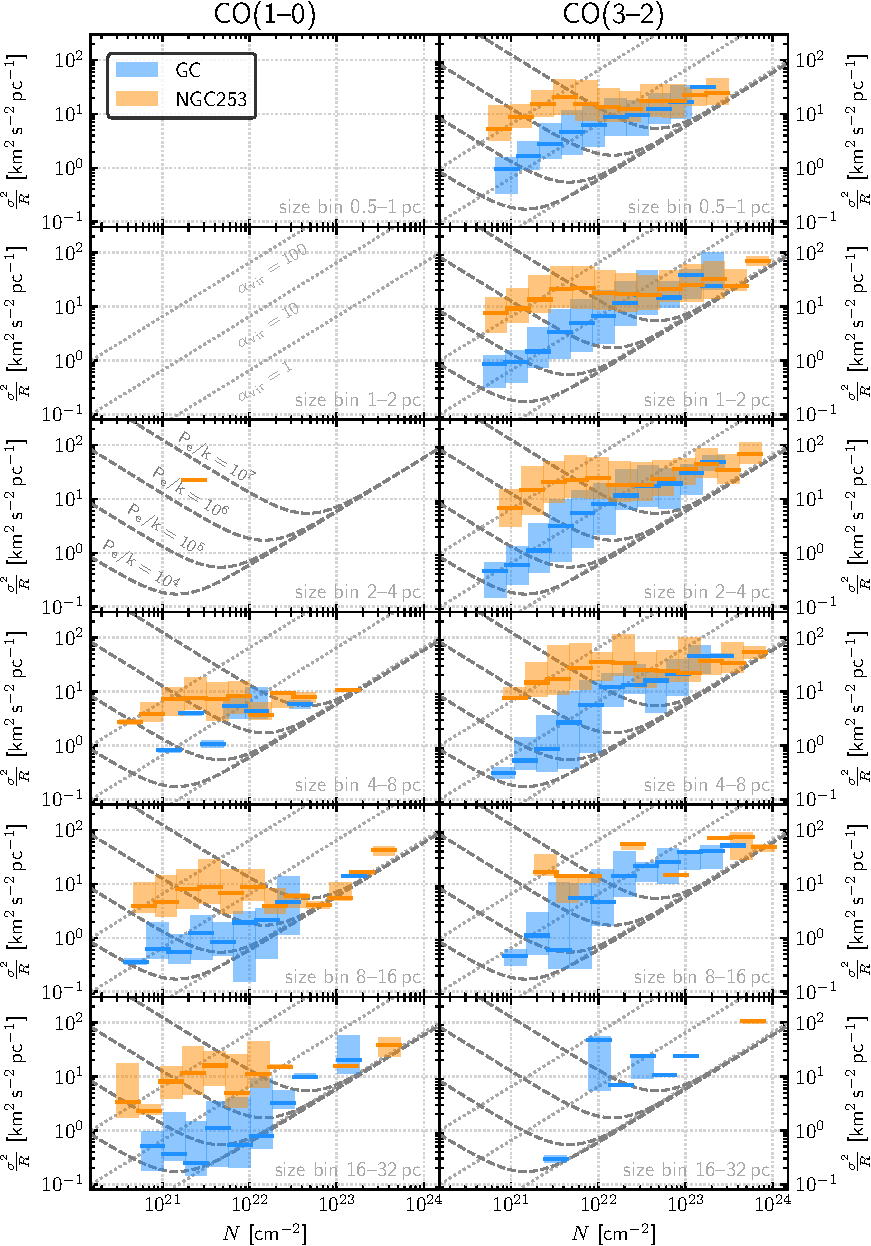
\includegraphics[width=\textwidth]{images/chapters/papers/dendro/dendro_figD}
    \caption[Size--line width coefficient vs. column density relation split by size]{Size--line width coefficient $\sigma^2/R$ as a function of column density for a range of structure size bins. \emph{left}: low resolution \co10; \emph{right}: high resolution \co32. The size bin for each panel is given in the lower right corner. Diagonal lines indicate constant virial parameters.
    \label{dendro: figure: D}}
\end{figure*}


%%%%%%%%%%%%%%%%%%%%%%%%%%%%%%%%%%%%%%%%%%%%%%%%%%%%%%%%%%%%%%%%%%%%%%%%%%%%%%%%%%%%%%%%%%%%%%%%%%%%